\documentclass[10pt]{article}
\usepackage[english]{babel}
\usepackage{../../../../lib/tex/naproche}
\usepackage{amssymb}
\usepackage{mathtools} % for \coloneq

\usepackage{stex-highlighting}
\providebool{emph} % "\newbool{emph}" does not work...
\setbool{emph}{false}
\colorlet{emphcolor}{violet}
\let\oldemph\emph
\renewcommand\emph[1]{\setbool{emph}{true}\ifbool{forthel}{\textcolor{emphcolor}{\itshape#1}}{\oldemph{#1}}\setbool{emph}{false}}
\renewcommand{\varemph}[1]{\ifbool{emph}{\textcolor{emphcolor}{#1}}{\textcolor{black}{#1}}}

\usepackage[right=6cm,left=3cm,bottom=3cm,marginparwidth=5cm]{geometry}

\usepackage{fancyhdr}
\renewcommand{\sectionmark}[1]{\markboth{#1}{}} 
\def\libarchive{}
\pagestyle{fancy}
\fancyhead[L]{\libarchive}
\fancyhead[C]{\nouppercase\leftmark}  % section title
\fancyhead[R]{\thepage}               % page number
\fancyfoot[C]{}                       % No page number in footer

\usepackage[nobottomtitles]{titlesec}
\titlespacing*{\section}{0pt}{30pt}{0pt}
\titlespacing*{\subsection}{0pt}{30pt}{0pt}
\titlespacing*{\subsubsection}{0pt}{30pt}{0pt}

\documentclass[12pt,oneside]{book}

\usepackage[foundations]{../../lib/tex/naproche}
\usepackage{../../lib/tex/libraries}
\usepackage{graphicx}
\usepackage{float}
\usepackage{caption}
\usepackage{footnote}

\makesavenoteenv{tabular} % Make footnotes work in tabular environments


\title{Foundations of Mathematics}
\author{Marcel Schütz}
\date{2022}

\begin{document}
  \maketitle

  \tableofcontents

  \begin{figure}[H]
    \centering
    \fbox{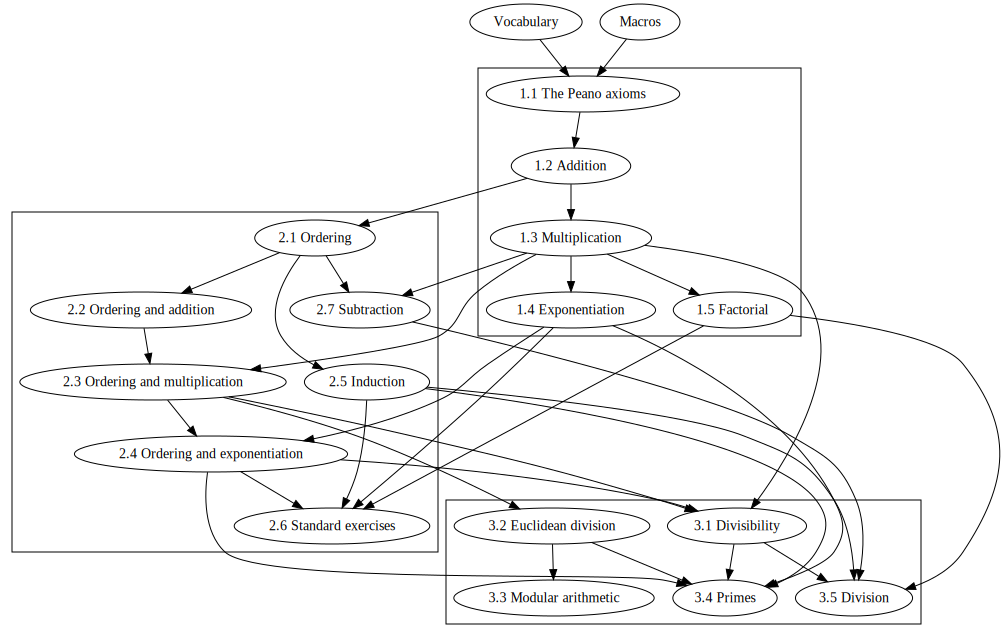
\includegraphics[width=0.9\linewidth]{./dependency-graph/graph.png}}
    \caption*{Interdependencies of the chapters}
  \end{figure}


  \section*{Introduction}

  This is a library providing a foundation of mathematics based on a
  Kelley-Morse like class theory with urelements.
  It introduces common operations on classes like unions or intersections
  (\cref{chapter:classes}) together with detailed proofs of their algebraic
  properties (\cref{chapter:computation-laws-for-classes}), the symmetric
  difference of two classes (\cref{chapter:symmetric-difference}) and the
  notions of ordered pairs and Cartesian products
  (\cref{chapter:pairs-and-products}) as well as proofs of the algebraic
  properties of the latter (\cref{chapter:computation-laws-for-products}).
  Moreover, it provides common operations on maps (\cref{chapter:maps}), various
  properties of images and preimages (\cref{chapter:image-and-preimage}) and the
  notions of injectivity, surjectivity, bijectivity
  (\cref{chapter:injections-surjections-bijections}) and invertibility of maps
  (\cref{chapter:invertible-maps}).
  The library provides an axiom system characterizing sets (\cref{chapter:sets})
  and, furthermore, it covers the notions of binary relations
  (\cref{chapter:binary-relations}), fixed-points of subset preserving maps
  (\cref{chapter:fixed-points}), including and equinumerosity
  (\cref{chapter:equinumerosity}).

  As two famous results it includes the Knaster-Tarski fixed point theorem
  (\cref{FOUNDATIONS_12_8420450166112256}) and the Cantor-Schröder-Bernstein
  theorem (\cref{FOUNDATIONS_13_1913663275401216}).

  \paragraph*{Usage.}
  At the very beginning of each chapter you can find the name of its source
  file, e.g. \path{foundations/sections/01_classes.ftl.tex} for
  \cref{chapter:classes}. This filename can be used to import the chapter via
  \Naproche's \texttt{readtex} instruction to another ForTheL text, e.g.:
  \begin{center}
    \verb`[readtex \path{foundations/sections/01_classes.ftl.tex}]`
  \end{center}

  \paragraph*{Checking times.}
  The checking times for each of the chapters may vary from computer to
  computer, but on mid-range hardware they are likely to be similar to those
  given in table below:

  \begin{center}
    \begin{tabular}{c|c|c}

      & \multicolumn{2}{c}{\textbf{Checking time}}
      \\
      \textbf{Chapter}
      & \textbf{without dependencies}     & \textbf{with dependencies}
      \\ \hline
      \ref{chapter:classes}
      & 00:04 min                         & 00:04 min
      \\
      \ref{chapter:computation-laws-for-classes}
      & 00:12 min                         & 00:16 min
      \\
      \ref{chapter:symmetric-difference}
      & 00:32 min                         & 00:48 min
      \\
      \ref{chapter:pairs-and-products}
      & 00:08 min                         & 00:12 min
      \\
      \ref{chapter:computation-laws-for-products}
      & 01:36 min                         & 01:56 min
      \\
      \ref{chapter:maps}
      & 01:13 min                         & 01:25 min
      \\
      \ref{chapter:image-and-preimage}
      & 01:28 min                         & 02:53 min
      \\
      \ref{chapter:injections-surjections-bijections}
      & 00:38 min                         & 02:03 min
      \\
      \ref{chapter:invertible-maps}
      & 02:20 min                         & 04:23 min
      \\
      \ref{chapter:sets}
      & 02:17 min                         & 06:40 min
      \\
      \ref{chapter:binary-relations}
      & 00:14 min                         & 06:54 min
      \\
      \ref{chapter:fixed-points}
      & 00:33 min                         & 07:13 min
      \\
      \ref{chapter:equinumerosity}
      & 01:48 min                         & 09:01 min
    \end{tabular}
  \end{center}


  \subfile{sections/01_classes.ftl.tex}
  \subfile{sections/02_computation-laws-for-classes.ftl.tex}
  \subfile{sections/03_symmetric-difference.ftl.tex}
  \subfile{sections/04_pairs-and-products.ftl.tex}
  \subfile{sections/05_computation-laws-for-products.ftl.tex}
  \subfile{sections/06_maps.ftl.tex}
  \subfile{sections/07_image-and-preimage.ftl.tex}
  \subfile{sections/08_injections-surjections-bijections.ftl.tex}
  \subfile{sections/09_invertible-maps.ftl.tex}
  \subfile{sections/10_sets.ftl.tex}
  \subfile{sections/11_binary-relations.ftl.tex}
  \subfile{sections/12_fixed-points.ftl.tex}
  \subfile{sections/13_equinumerosity.ftl.tex}
\end{document}

\usepackage{amssymb}

\newcommand{\Nat}{\mathbb{N}}
\newcommand{\Prime}{\mathbb{P}}
\renewcommand{\succ}{\textrm{succ}}
\newcommand{\pred}{\textrm{pred}}
\newcommand{\add}{\textrm{add}}
\newcommand{\mul}{\textrm{mul}}
\renewcommand{\exp}{\textrm{exp}}
\newcommand{\fac}{\textrm{fac}}
\renewcommand{\div}{\mathop{\textrm{div}}}
\renewcommand{\mod}{\mathop{\textrm{mod}}}

\begin{document}
  \begin{imports}
    \begin{forthel}
      %[prove off][check off]
      [readtex \path{libraries/source/arithmetics/06_multiplication.ftl.tex}]
      %[prove on][check on]
    \end{forthel}
  \end{imports}


  \section{Definition of Exponentiation}

  \begin{forthel}
    \begin{signature}\printlabel{ARITHMETIC_13_3663815629602816}
      Let $n, m$ be natural numbers.
      $n^{m}$ is a natural number.
    \end{signature}
  \end{forthel}

  \begin{forthel}
    \begin{axiom}\printlabel{ARITHMETIC_13_5368818025103360}
      Let $n$ be a natural number.
      Then $n^{0} = 1$.
    \end{axiom}
  \end{forthel}

  \begin{forthel}
    \begin{axiom}\printlabel{ARITHMETIC_13_4140498660884480}
      Let $n, m$ be natural numbers.
      Then $n^{m + 1} = n^{m} \cdot n$.
    \end{axiom}
  \end{forthel}


  \section{Computation Laws}

  \subsection{Exponentiation with $0$, $1$ and $2$}

  \begin{forthel}
    \begin{proposition}\printlabel{ARITHMETIC_13_4673644676513792}
      Let $n$ be a natural number.
      Assume $n \neq 0$.
      Then \[ 0^{n} = 0. \]
    \end{proposition}
    \begin{proof}
      Take a natural number $m$ such that $n = m + 1$.
      Then $0^{n}
        = 0^{m + 1}
        = 0^{m} \cdot 0
        = 0$.
      Indeed $0^{m + 1} = 0^{m} \cdot 0$ (by \cref{ARITHMETIC_13_4140498660884480}).
    \end{proof}
  \end{forthel}

  \begin{forthel}
    \begin{proposition}\printlabel{ARITHMETIC_13_7376849881530368}
      Let $n$ be a natural number.
      Then \[ 1^{n} = 1. \]
    \end{proposition}
    \begin{proof}
      Define $\Phi = \{ n' \in \Nat \mid 1^{n'} = 1 \}$.

      (1) $\Phi$ contains $0$.

      (2) For all $n' \in \Phi$ we have $n' + 1 \in \Phi$. \\
      Proof.
        Let $n' \in \Phi$.
        Then $1^{n' + 1}
          = 1^{n'} \cdot 1
          = 1 \cdot 1
          = 1$.
      Qed.

      Hence every natural number is contained in $\Phi$ (by \cref{ARITHMETIC_03_647949900054528}).
      Thus $1^{n} = 1$.
    \end{proof}
  \end{forthel}

  \begin{forthel}
    \begin{proposition}\printlabel{ARITHMETIC_13_4975279749464064}
      Let $n$ be a natural number.
      Then \[ n^{1} = n. \]
    \end{proposition}
    \begin{proof}
      We have $n^{1}
        = n^{0 + 1}
        = n^{0} \cdot n
        = 1 \cdot n
        = n$.
    \end{proof}
  \end{forthel}

  \begin{forthel}
    \begin{proposition}\printlabel{ARITHMETIC_13_8513812055457792}
      Let $n$ be a natural number.
      Then \[ n^{2} = n \cdot n. \]
    \end{proposition}
    \begin{proof}
      We have $n^{2}
        = n^{1 + 1}
        = n^{1} \cdot n
        = n \cdot n$.
    \end{proof}
  \end{forthel}


  \subsection{Sums as Exponents}

  \begin{forthel}
    \begin{proposition}\printlabel{ARITHMETIC_13_8152207530655744}
      Let $n, m, k$ be natural numbers.
      Then \[ k^{n + m} = k^{n} \cdot k^{m}. \]
    \end{proposition}
    \begin{proof}
      Define $\Phi = \{ m' \in \Nat \mid k^{n + m'} = k^{n} \cdot k^{m'} \}$.

      (1) $\Phi$ contains $0$. \\
      Indeed $k^{n + 0}
        = k^{n}
        = k^{n} \cdot 1
        = k^{n} \cdot k^{0}$.

      (2) For all $m' \in \Phi$ we have $m' + 1 \in \Phi$. \\
      Proof.
        Let $m' \in \Phi$.
        Then
        \[  k^{n + (m' + 1)}                  \]
        \[    = k^{(n + m') + 1}              \]
        \[    = k^{n + m'} \cdot k            \]
        \[    = (k^{n} \cdot k^{m'}) \cdot k  \]
        \[    = k^{n} \cdot (k^{m'} \cdot k)  \]
        \[    = k^{n} \cdot k^{m' + 1}.       \]
      Qed.

      Hence every natural number is contained in $\Phi$ (by \cref{ARITHMETIC_03_647949900054528}).
      Thus $k^{n + m} = k^{n} \cdot k^{m}$.
    \end{proof}
  \end{forthel}


  \subsection{Products as Exponents}

  \begin{forthel}
    \begin{proposition}\printlabel{ARITHMETIC_13_7827956571308032}
      Let $n, m, k$ be natural numbers.
      Then \[ n^{m \cdot k} = (n^{m})^{k}. \]
    \end{proposition}
    \begin{proof}
      Define $\Phi = \{ k' \in \Nat \mid n^{m \cdot k'} = (n^{m})^{k'} \}$.

      (1) $\Phi$ contains $0$.
      Indeed $(n^{m})^{0}
        = 1
        = n^{0}
        = n^{m \cdot 0}$.

      (2) For all $k' \in \Phi$ we have $k' + 1 \in \Phi$. \\
      Proof.
        Let $k' \in \Phi$.
        Then
        \[  (n^{m})^{k' + 1}                \]
        \[    = (n^{m})^{k'} \cdot n^{m}    \]
        \[    = n^{m \cdot k'} \cdot n^{m}  \]
        \[    = n^{(m \cdot k') + m}        \]
        \[    = n^{m \cdot (k' + 1)}.       \]
      Qed.

      Therefore every natural number is contained in $\Phi$ (by \cref{ARITHMETIC_03_647949900054528}).
      Consequently $n^{m \cdot k} = (n^{m})^{k}$.
    \end{proof}
  \end{forthel}


  \subsection{Products as Base}

  \begin{forthel}
    \begin{proposition}\printlabel{ARITHMETIC_13_2563032276271104}
      Let $n, m, k$ be natural numbers.
      Then \[ (n \cdot m)^{k} = n^{k} \cdot m^{k}. \]
    \end{proposition}
    \begin{proof}
      Define $\Phi = \{ k' \in \Nat \mid (n \cdot m)^{k'} =
      n^{k'} \cdot m^{k'} \}$.

      (1) $\Phi$ contains $0$.
      Indeed $((n \cdot m)^{0})
        = 1
        = 1 \cdot 1
        = n^{0} \cdot m^{0}$. %!

      (2) For all $k' \in \Phi$ we have $k' + 1 \in \Phi$. \\
      Proof.
        Let $k' \in \Phi$.

        Let us show that $(n^{k'} \cdot m^{k'}) \cdot (n \cdot m) =
        (n^{k'} \cdot n) \cdot (m^{k'} \cdot m)$.
          \[  (n^{k'} \cdot m^{k'}) \cdot (n \cdot m)       \]
          \[    = ((n^{k'} \cdot m^{k'}) \cdot n) \cdot m   \]
          \[    = (n^{k'} \cdot (m^{k'} \cdot n)) \cdot m   \]
          \[    = (n^{k'} \cdot (n \cdot m^{k'})) \cdot m   \]
          \[    = ((n^{k'} \cdot n) \cdot m^{k'}) \cdot m   \]
          \[    = (n^{k'} \cdot n) \cdot (m^{k'} \cdot m).  \]
        Qed.

        Hence
        \[  (n \cdot m)^{k' + 1}                          \]
        \[    = (n \cdot m)^{k'} \cdot (n \cdot m)        \]
        \[    = (n^{k'} \cdot m^{k'}) \cdot (n \cdot m)   \]
        \[    = (n^{k'} \cdot n) \cdot (m^{k'} \cdot m)   \]
        \[    = n^{k' + 1} \cdot m^{k' + 1}.              \]
      Qed.

      Therefore every natural number is contained in $\Phi$ (by \cref{ARITHMETIC_03_647949900054528}).
      Consequently $(n \cdot m)^{k} = n^{k} \cdot m^{k}$.
    \end{proof}
  \end{forthel}


  \subsection{Zeroes of Exponentiation}

  \begin{forthel}
    \begin{proposition}\printlabel{ARITHMETIC_13_3860221447372800}
      Let $n, m$ be natural numbers.
      Then \[ n^{m} = 0 \iff (\text{$n = 0$ and $m \neq 0$}). \]
    \end{proposition}
    \begin{proof}
      Case $n^{m} = 0$.
        Define $\Phi = \{ m' \in \Nat \mid$ if $n^{m'} = 0$ then $n = 0$ and
        $m' \neq 0 \}$.

        (1) $\Phi$ contains $0$.
        Indeed if $n^{0} = 0$ then we have a contradiction.

        (2) For all $m' \in \Phi$ we have $m' + 1 \in \Phi$. \\
        Proof.
          Let $m' \in \Phi$.

          Let us show that if $n^{m' + 1} = 0$ then $n = 0$ and $m' + 1 \neq 0$.
            Assume $n^{m' + 1} = 0$.
            Then $0 = n^{m' + 1} = n^{m'} \cdot n$.
            Hence $n^{m'} = 0$ or $n = 0$.
            We have $m' + 1 \neq 0$ and if $n^{m'} = 0$ then $n = 0$.
            Hence $n = 0$ and $m' + 1 \neq 0$.
          End.
        Qed.

        Thus every natural number is contained in $\Phi$ (by \cref{ARITHMETIC_03_647949900054528}).
        Consequently $m \in \Phi$.
        Therefore $n = 0$ and $m \neq 0$.
      End.

      Case $n = 0$ and $m \neq 0$.
        Take a natural number $k$ such that $m = k + 1$.
        Then $n^{m}
          = n^{k + 1}
          = n^{k} \cdot n
          = 0^{k} \cdot 0
          = 0$.
      End.
    \end{proof}
  \end{forthel}


  \section{Ordering and Exponentiation}

  \begin{forthel}
    \begin{proposition}\printlabel{ARITHMETIC_13_3373702288769024}
      Let $n, m, k$ be natural numbers.
      Assume $k \neq 0$.
      Then \[ n < m \iff n^{k} < m^{k}. \]
    \end{proposition}
    \begin{proof}
      Case $n < m$.
        Define $\Phi = \{ k' \in \Nat \mid$ if $k' > 1$ then
        $n^{k'} < m^{k'} \}$.

        (1) $\Phi$ contains $0$.

        (2) $\Phi$ contains $1$.

        (3) $\Phi$ contains $2$. \\
        Proof.
          Case $n = 0$ or $m = 0$. Obvious.

          Case $n, m \neq 0$.
            Then $n \cdot n
              < n \cdot m
              < m \cdot m$.
            Hence $n^{2}
              = n \cdot n
              < n \cdot m
              < m \cdot m
              = m^{2}$.
          End.
        Qed.

        (4) For all $k' \in \Phi$ we have $k' + 1 \in \Phi$. \\
        Proof.
          Let $k' \in \Phi$.

          Let us show that if $k' + 1 > 1$ then
          $n^{k' + 1} < m^{k' + 1}$.
            Assume $k' + 1 > 1$.
            Then $n^{k'} < m^{k'}$.
            Indeed $k' \neq 0$ and $if k' = 1$ then $n^{k'} < m^{k'}$.

            Case $k' \leq 1$.
              Then $k' = 0$ or $k' = 1$.
              Hence $k' + 1 = 1$ or $k' + 1 = 2$.
              Thus $k' + 1 \in \Phi$.
              Therefore $n^{k' + 1} < m^{k' + 1}$.
            End.

            Case $k' > 1$.
              Case $n = 0$.
                Then $m \neq 0$.
                Hence $n^{k' + 1}
                  = 0
                  < m^{k'} \cdot m
                  = m^{k' + 1}$.
                Thus $n^{k' + 1} < m^{k' + 1}$.
              End.

              Case $n \neq 0$.
                Then $n^{k'} \cdot n
                  < m^{k'} \cdot n
                  < m^{k'} \cdot m$.
                Indeed $n^{k'} < m^{k'} \neq 0$.
                Take $A = n^{k' + 1}$ and $B = m^{k' + 1}$. %!
                Then $A
                  = n^{k' + 1}
                  = n^{k'} \cdot n
                  < m^{k'} \cdot n
                  < m^{k'} \cdot m
                  = m^{k' + 1}
                  = B$.
                Thus $n^{k' + 1} = A < B = m^{k' + 1}$.
              End.
            End.

            Hence $n^{k' + 1} < m^{k' + 1}$.
            Indeed $k' \leq 1$ or $k' > 1$.
          End.

          Thus $k' + 1 \in \Phi$.
        Qed.

        Therefore every natural number is contained in $\Phi$ (by \cref{ARITHMETIC_03_647949900054528}).
        Consequently $n^{k} < m^{k}$.
      End.

      Case $n^{k} < m^{k}$.
        Define $\Psi = \{ k' \in \Nat \mid$ if $n \geq m$ then
        $n^{k'} \geq m^{k'} \}$.

        (1) $\Psi$ contains $0$.

        (2) For all $k' \in \Psi$ we have $k' + 1 \in \Psi$. \\
        Proof.
          Let $k' \in \Psi$.

          Let us show that if $n \geq m$ then $n^{k' + 1} \geq m^{k' + 1}$.
            Assume $n \geq m$.
            Then $n^{k'} \geq m^{k'}$.
            Hence $n^{k'} \cdot n \geq m^{k'} \cdot n \geq m^{k'} \cdot m$.
            Take $A = n^{k' + 1}$ and $B = m^{k' + 1}$. %!
            Thus $A
              = n^{k' + 1}
              = n^{k'} \cdot n
              \geq m^{k'} \cdot n
              \geq m^{k'} \cdot m
              = m^{k' + 1}
              = B$.
            Therefore $n^{k' + 1} = A \geq B = m^{k' + 1}$.
          End.

          Hence $k' + 1 \in \Psi$.
        Qed.

        Thus every natural number is contained in $\Psi$ (by \cref{ARITHMETIC_03_647949900054528}).
        Therefore if $n \geq m$ then $n^{k} \geq m^{k}$.
        Consequently $n < m$.
      End.
    \end{proof}
  \end{forthel}

  \begin{forthel}
    \begin{corollary}\printlabel{ARITHMETIC_13_2797602550579200}
      Let $n, m, k$ be natural numbers.
      Assume $k \neq 0$.
      Then \[ n^{k} = m^{k} \implies n = m. \]
    \end{corollary}
    \begin{proof}
      Assume $n^{k} = m^{k}$.
      Suppose $n \neq m$.
      Then $n < m$ or $m < n$.
      If $n < m$ then $n^{k} < m^{k}$.
      If $m < n$ then $m^{k} < n^{k}$.
      Thus $n^{k} \neq m^{k}$.
      Contradiction.
    \end{proof}
  \end{forthel}

  \begin{forthel}
    \begin{corollary}\printlabel{ARITHMETIC_13_6875081963732992}
      Let $n, m, k$ be natural numbers.
      Assume $k \neq 0$.
      Then \[ n^{k} \leq m^{k} \iff n \leq m. \]
    \end{corollary}
    \begin{proof}
      If $n^{k} < m^{k}$ then $n < m$.
      If $n^{k} = m^{k}$ then $n = m$.
      [prover vampire]
      Hence $n^{k} \leq m^{k} \implies n \leq m$.
      [prover eprover]

      If $n < m$ then $n^{k} < m^{k}$.
      If $n = m$ then $n^{k} = m^{k}$.
      Hence $n \leq m \implies n^{k} \leq m^{k}$.
    \end{proof}
  \end{forthel}

  \begin{forthel}
    \begin{proposition}\printlabel{ARITHMETIC_13_3349764703780864}
      Let $n, m, k$ be natural numbers.
      Assume $k > 1$.
      Then \[ n < m \iff k^{n} < k^{m}. \]
    \end{proposition}
    \begin{proof}
      Case $n < m$.
        Define $\Phi = \{ m' \in \Nat \mid$ if $n < m'$ then
        $k^{n} < k^{m'} \}$.

        (1) $\Phi$ contains $0$.

        (2) For all $m' \in \Phi$ we have $m' + 1 \in \Phi$. \\
        Proof.
          Let $m' \in \Phi$.

          Let us show that if $n < m' + 1$ then $k^{n} < k^{m' + 1}$.
            Assume $n < m' + 1$.
            Then $n \leq m'$.
            We have $k^{m'} \cdot 1 < k^{m'} \cdot k$.
            Indeed $k^{m'} \neq 0$.

            Case $n = m'$.
              Take $A = k^{n}$ and $B = k^{m' + 1}$. %!
              Then $A
                = k^{n}
                = k^{m'}
                < k^{m'} \cdot k
                = k^{m' + 1}
                = B$.
              Hence $k^{n} = A < B = k^{m' + 1}$.
            End.

            Case $n < m'$.
              Take $A = k^{n}$ and $B = k^{m' + 1}$. %!
              Then $A
                = k^{n}
                < k^{m'}
                < k^{m'} \cdot k
                = k^{m' + 1}
                = B$.
              Hence $k^{n} = A < B = k^{m' + 1}$.
            End.
          Qed.
        Qed.

        Hence every natural number is contained in $\Phi$ (by \cref{ARITHMETIC_03_647949900054528}).
        Thus $k^{n} < k^{m}$.
      End.

      Case $k^{n} < k^{m}$.
        Define $\Psi = \{ n' \in \Nat \mid$ if $n' \geq m$ then
        $k^{n'} \geq k^{m} \}$.

        (1) $0$ is contained in $\Psi$.

        (2) For all $n' \in \Psi$ we have $n' + 1 \in \Psi$. \\
        Proof.
          Let $n' \in \Psi$.

          Let us show that if $n' + 1 \geq m$ then $k^{n' + 1} \geq k^{m}$.
            Assume $n' + 1 \geq m$.

            Case $n' + 1 = m$. Obvious.

            Case $n' + 1 > m$.
              Then $n' \geq m$.
              Hence $k^{n'} \geq k^{m}$.
              We have $k^{n'} \cdot 1 \leq k^{n'} \cdot k$.
              Indeed $1 \leq k$ and $k^{n'} \neq 0$.
              Take $A = k^{m}$ and $B = k^{n' + 1}$. %!
              Then $A
                = k^{m}
                \leq k^{n'}
                = k^{n'} \cdot 1
                \leq k^{n'} \cdot k
                = k^{n' + 1}
                = B$.
              Hence $k^{m} = A \leq B = k^{n' + 1}$.
            End.
          Qed.
        Qed.

        Thus every natural number is contained in $\Psi$ (by \cref{ARITHMETIC_03_647949900054528}).
        Therefore if $n \geq m$ then $k^{n} \geq k^{m}$.
        [prover vampire]
        Consequently $n < m$.
      End.
    \end{proof}
  \end{forthel}

  \begin{forthel}
    \begin{corollary}\printlabel{ARITHMETIC_13_6780506905509888}
      Let $n, m, k$ be natural numbers.
      Assume $k > 1$.
      Then \[ k^{n} = k^{m} \implies n = m. \]
    \end{corollary}
    \begin{proof}
      Assume $k^{n} = k^{m}$.
      Suppose $n \neq m$.
      Then $n < m$ or $m < n$.
      If $n < m$ then $k^{n} < k^{m}$.
      If $m < n$ then $k^{m} < k^{n}$.
      Thus $k^{n} \neq k^{m}$.
      Contradiction.
    \end{proof}
  \end{forthel}

  \begin{forthel}
    \begin{corollary}\printlabel{ARITHMETIC_13_2876620253691904}
      Let $n, m, k$ be natural numbers.
      Assume $k > 1$.
      Then \[ n \leq m \iff k^{n} \leq k^{m}. \]
    \end{corollary}
    \begin{proof}
      If $n \leq m$ then $k^{n} \leq k^{m}$.

      Let us show that if $k^{n} \leq k^{m}$ then $n \leq m$.
        Case $k^{n} = k^{m}$. Obvious (by \cref{ARITHMETIC_13_6780506905509888}).
        Case $k^{n} < k^{m}$. Obvious.
      End.
    \end{proof}
  \end{forthel}

  \begin{forthel}
    \begin{proposition}\printlabel{ARITHMETIC_13_6984104377581568}
      Let $n$ be a natural number.
      Then \[ (n + 1)^{2} = (n^{2} + (2 \cdot n)) + 1. \]
    \end{proposition}
    \begin{proof}
      We have
      \[  (n + 1)^{2}                       \]
      \[    = (n + 1) \cdot (n + 1)         \]
      \[    = ((n + 1) \cdot n) + (n + 1)   \]
      \[    = ((n \cdot n) + n) + (n + 1)   \]
      \[    = (n^{2} + n) + (n + 1)         \]
      \[    = ((n^{2} + n) + n) + 1         \]
      \[    = (n^{2} + (n + n)) + 1         \]
      \[    = (n^{2} + (2 \cdot n)) + 1.    \]
    \end{proof}
  \end{forthel}

  \begin{forthel}
    \begin{proposition}\printlabel{ARITHMETIC_13_134060414337024}
      Let $n$ be a natural number.
      Assume $n \geq 3$.
      Then \[ n^{2} > (2 \cdot n) + 1. \]
    \end{proposition}
    \begin{proof}
      Define $\Phi = \{ n' \in \Nat_{\geq 3} \mid n'^{2} > (2 \cdot n') + 1 \}$.

      (1) $\Phi$ contains $3$.
      Indeed $3^{2} > (2 \cdot 3) + 1$.

      (2) For all $n' \in \Phi$ we have $n' + 1 \in \Phi$. \\
      Proof.
        Let $n' \in \Phi$.
        Then $n' \geq 3$.

        (a) $(n'^{2} + (2 \cdot n')) + 1
        > (((2 \cdot n') + 1) + (2 \cdot n')) + 1$.
        Indeed $n'^{2} + (2 \cdot n') > ((2 \cdot n') + 1) + (2 \cdot n')$.

        (b) $(((2 \cdot n') + 1) + (2 \cdot n')) + 1
        > ((2 \cdot n') + (2 \cdot n')) + 1$. \\
        Proof.
          We have $((2 \cdot n') + 1) + (2 \cdot n')
          > (2 \cdot n') + (2 \cdot n')$.
          Indeed $(2 \cdot n') + 1 > 2 \cdot n'$.
        Qed.

        (c) $(2 \cdot (n' + n')) + 1 > (2 \cdot (n' + 1)) + 1$. \\
        Proof.
          We have $n' + n' > n' + 1$ and $2 \neq 0$.
          Thus $2 \cdot (n' + n') > 2 \cdot (n' + 1)$ (by \cref{ARITHMETIC_06_5048640368279552}).
          Indeed $n' + n'$ and $n' + 1$ are natural numbers.
        Qed.

        Take $A = (n' + 1)^{2}$ and $B = (2 \cdot (n' + 1)) + 1$. %!
        Then
        \[  A                                             \]
        \[    = (n' + 1)^{2}                              \]
        \[    = (n'^{2} + (2 \cdot n')) + 1               \]
        \[    > (((2 \cdot n') + 1) + (2 \cdot n')) + 1   \]  % (a)
        \[    > ((2 \cdot n') + (2 \cdot n')) + 1         \]  % (b)
        \[    = (2 \cdot (n' + n')) + 1                   \]
        \[    > (2 \cdot (n' + 1)) + 1                    \]  % (c)
        \[    = B.                                        \]

        Thus $(n' + 1)^{2} = A > B = (2 \cdot (n' + 1)) + 1$.
      Qed.

      [prover vampire]
      Therefore $\Phi$ contains every element of $\Nat_{\geq 3}$ (by \cref{ARITHMETIC_04_4976599269113856}, 1, 2).
      [prover eprover]
      Consequently $n^{2} > (2 \cdot n) + 1$.
    \end{proof}
  \end{forthel}
\end{document}
